Here we consider the case in wich all the parameters are known and the goal is to maximize the cumulative expected reward, following a greedy approach.\\
The algorithm works as follow:
\begin{enumerate}
    \item set the prices of all the pruducts with the lowest one
    \item collect the reward obtained by increasing, each time, the price of just one product of the original super arm
    \item compare the five different configuration obtained with the first one. There could be two case\begin{enumerate}
        \item there is an increase of the reward, so select the one that gave the maximum reward (the highest increase) as the best one and repeat the algorithm from point 2
        \item there is no increse (all the new configuration is worst than the previous one) and stop the algoritm 
    \end{enumerate}
    \item Return the actual best configuration.
\end{enumerate}



\subsection{Results}
\begin{figure}[ht]
    \begin{center}
    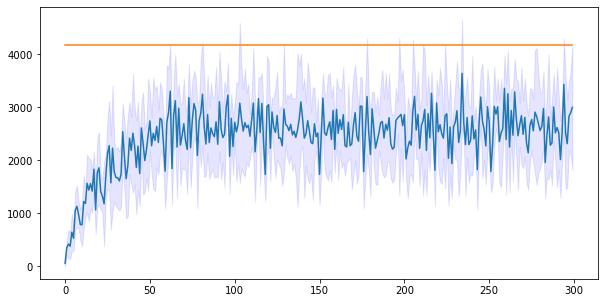
\includegraphics[width=0.6\textwidth]{img/reward2.png}
    \caption{Reward}
    \label{fig:reward2}
    \end{center}
\end{figure}
\begin{multicols}{2}
    \begin{figure}[H]
        \begin{center}
        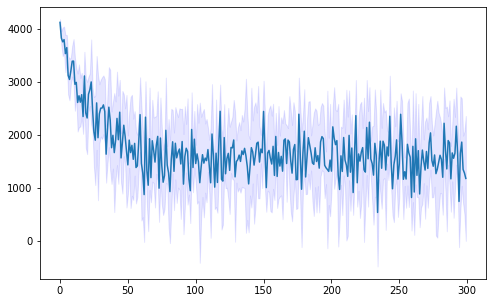
\includegraphics[width=0.5\textwidth]{img/regret2.png}
        \caption{Regret}
        \label{fig:regret2}
        \end{center}
    \end{figure}
    \columnbreak
    \begin{figure}[H]
        \begin{center}
        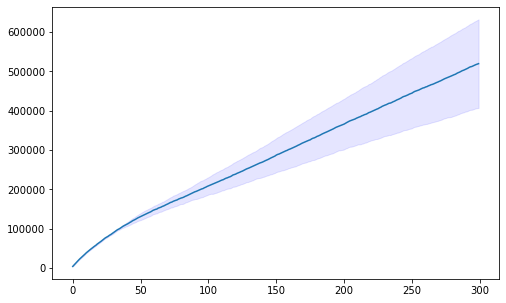
\includegraphics[width=0.5\textwidth]{img/cum_regret2.png}
        \caption{Cumulative regret}
        \label{fig:cum_reg2}
        \end{center}
    \end{figure}
\end{multicols}
